\documentclass[12pt]{amsart}
\usepackage[T1]{fontenc}
\usepackage{caption}
\usepackage{subcaption}
\usepackage[utf8]{inputenc}
\usepackage{fullpage}
\usepackage{parskip}
\usepackage{enumitem}
\usepackage[english]{babel}
\usepackage{biblatex}
\usepackage{hyperref}
\usepackage{amsmath,amssymb,amsthm, amsfonts}
\usepackage{graphicx} 

\graphicspath{ {./images/} }
\addbibresource{bibliography.bib}

\renewcommand\thesection{\Roman{section}}
\setcounter{section}{0}
\renewcommand\thesubsection{(\Roman{subsection})}
\renewcommand\theequation{\arabic{equation}}

\title{Depth reconstruction using stereo images}
\author{Gabriele Esposito\\964431}

\begin{document}
\setlength{\parskip}{0pt} % 1ex plus 0.5ex minus 0.2ex}
\setlength{\parindent}{0pt}
\maketitle
\section*{Objective}
The objective of the project is to retrieve relative depth information from a pair of stereo images using epipolar geometry and a minimal setup consisting of a 
single calibrated camera and no information on the portrayed scene. 
The two pictures of the same scene are shot using the same camera translated in space (and possibly rotated). The approach can be considered a
simple case of "Structure From Motion" using just two views of the same stationary object. A natural extension of this can be the introduction of multiple views to better reconstruct 
the 3D shape of the scene.
\section*{Approach}
The approach can be broken down into a sequence of steps:
\begin{enumerate}[label={\arabic*.}]
    \item Camera Calibration (to be performed just once for any new camera that needs to be used).
    \item Undistortion of stereo pair and intrinsic parameters update.
    \item Sparse matching.
        \begin{itemize} 
            \item Keypoints and descriptors computation (e.g. using SIFT).
            \item Keypoints matching.
        \end{itemize}
    \item Estimation of Fundamental matrix.
    \item Computation of Essential matrix with known intrinsic parameters and Fundamental matrix.
    \item Essential matrix decomposition through SVD.
    \item Stereo pair rectification.
    \item Disparity map computation using Stereo Block Matching on rectified images (dense correspondence).
    \item 3D reprojection (up to scale) of points with their estimated depth acquired from disparity.
\end{enumerate}
The output of this process is a color point cloud representing the 3D structure of the photographed scene (up to scale).
The following sections will address each step in more detail.
\subsection{Camera Calibration} \label{sec:calibration}
Calibration is performed using multiple views of a checkerboard pattern acquired with the camera to be calibrated, maintaining the same focus throughout all the shots.
The calibration process is comprised of the following steps for each of the calibration images:
\begin{enumerate}[label={\arabic*.}]
    \item Image resize to a fixed percentage of the original image size (circa 1000 x 700)
    \item Colorspace conversion (to HSV) and application of a mask to extract checkerboard pattern. 
    The mask values strongly depend on the brightness of the checkerboard with respect to the surrounding context.
    \item Morphology dilation with a rectangular pattern on the previously obtained mask.
    \item Checkerboard corners are found through the use of openCV \texttt{findChessboardCorners} function
    \item Chessboard corners position refinement through openCV \texttt{cornerSubPix}.
    \item Camera calibration (through OpenCV \texttt{calibrateCamera} \cite{calibration}) using object coordinates expressed with respect to a frame of reference centered at the top right corner of the pattern, 
    and relative image coordinates found with subpixel precision by \texttt{cornerSubPix}.
\end{enumerate}
This process outputs intrinsic parameters matrix: \[K = \left ( 
    \begin{array}{ c c c}
    f_x & 0   & x_0 \\
     0  & f_y & y_0 \\
     0  & 0   & 1 \\
    \end{array}
\right )\]
and distortion coefficients \((k_1, k_2, k_3, k_4, k_5)\) both later used to remove radial distortion and to rectify the two images.
Rotation and translation vectors (expressed in world coordinates w.r.t the pattern) albeit not used are also provided for each of the calibration images.
\\
Camera calibration is performed just once as the first step for each new camera that needs to be used, images containing a calibration pattern need to be supplied for any new camera.
\subsection{Preprocessing}
Once intrinsic parameters and distortion coefficients are obtained for the used camera, 
the two images of the stereo pair from which we want to extract scene depth are supplied and pre-processed.
\\
Each of the two images of the stereo pair is resized to the same shape as in the initial calibration procedure, this step is important because any other size would not match
with the calibration parameters found.
Radial distortion is removed from each of the two images of the stereo pair, 
and a new updated calibration matrix is returned to take into account the transformation performed.
Undistortion is performed using the camera's intrinsic parameters and distortion coefficients found during the calibration phase.
\subsection{Sparse Matching}
The relative position of the camera in the second shot with respect to the previous is found through the use of point correspondences in the two views as explained in the next section.
The matching points in the two views will correspond to the same 3D point in the scene.
\\To extract such matches, keypoints, and corresponding descriptors are computed on both images using the \textbf{Scale Invariant Feature Transform} algorithm.
In order to match the found keypoints according to their similarity different approaches can be used. The simplest solution is to find matches using a bruteforce approach,
this involves comparing every possible pair of matches to determine which ones are the most similar (smallest L2-norm), matches are then ranked in order of similarity and only the best ones are taken.
\\
A second and more efficient solution is to use the \textbf{FLANN-based matcher}. FLANN uses a different distance measure (Hellinger) instead of the classic L2-norm to compare SIFT descriptors, 
this leads to a dramatic improvement in speed. To filter matches Lowe's ratio test is used, which measures the distance ratio between the two nearest matches of any considered
keypoint, it is considered a good match when this value is below a threshold (often fixed between 0.7 and 0.8).
\\
An alternative approach to find matches is to select them manually in both images, this approach can be time consuming and does not allow to find a high number of matching points.
The following steps in the pipeline work best with a high number of matches found on multiple planes in the two views so this solution can be used in cases in which the automatic approach 
finds a high number of wrong matches. (e.g. images with repeating patterns, vast solid color areas).
\subsection{Fundamental matrix estimation}
To determine position of one camera relative to the other expressed as a rotation matrix \(R\) and a translation vector \(t\) epipolar geometry is used.
Specifically, the epipolar constraint allows us to compute \(E\) and \(F\) the Essential and Fundamental matrices from a finite number of correspondences in the two images as mentioned above.
The Fundamental matrix is used to derive the Essential matrix containing pose information.\\
The epipolar constraint is a geometrical constraint that can be written as:
\[[p_2; 1]^T K^{-T} E K^{-1} [p_1; 1] = 0\]
where \(E\) is an essential matrix, \(p_1\) and \(p_2\) are corresponding points in the first and the second images respectively,
and \(K\) are the intrinsic parameter matrices of the two cameras (in this setup they are identical since stereo pair is acquired with same camera).
\\
We know that: 
\[F = K^{-T} E K^{-1}\]
so we can write the epipolar constraint more simply as:
\[[p_2; 1]^T F [p_1; 1] = 0\]
In order to retrieve pose information we need to estimate the Fundamental matrix first from this epipolar constraint. 
To do so the implementation chosen (OpenCV) uses \textbf{Random Sample Consensus} (RANSAC), which iteratively estimates the most probable model parameters given the correspondences
found in earlier stages.\\
After estimating F it is easy to derive \(E\) and since we know that \(E = R[T_x]\) (where \([T_x]\) denotes the skew-symmetric matrix such that \([T_x]x = t \times x \) is the cross-product of the vectors t and x).
we can derive pose information through \textbf{Singular Value Decomposition} (SVD) on the Essential matrix.
The accuracy of this entire procedure estimating the pose of one camera with respect to the other heavily depends on the accuracy of the initial calibration procedure and
the quality and number of correspondences found in the two images.
\subsection{Dense correspondence}
We know from epipolar geometry that the projection of a scene point onto the first image generates a \textit{line} on the other image plane where the corresponding point must lie.
In this context finding the correspondence of a projected point onto the first image plane in the second image plane results in a 1D search on such epipolar line.
To solve the problem more practically a solution is to project both image planes onto a common plane parallel to the baseline joining the two optical centers. This process is known as 
\textit{rectification} and effectively makes epipolar lines parallel.\\
This is performed computing two rotation matrices one for each camera that will make both image planes virtually the same plane.\\ 
The procedure needs to use intrinsic parameters for both cameras together with pose information (\(K, R, t\)).
Now given two points \(p\) and \(p'\) located on the same scanline of the left and right images, with coordinates \((x, y)\) and \((x', y)\), 
the disparity is defined as the difference \[d = x' - x = \frac{Bf}{Z} \]
If B denotes the distance between the optical centers, also called the baseline in this context, 
the depth of P in the (normalized) coordinate system attached to the first camera is \[Z = -Bf/d\] 
In particular, the coordinate vector of the point P in the frame attached to the first camera is 
\(P = -(Bf/d)p\), where \(p = (x,y,1)^T\) is the vector of normalized image coordinates of p (see figure \ref{fig:disp}).
In short, the above equation says that the depth of a point in a scene is inversely proportional to the difference in distance of corresponding image points and their camera centers. 
So to find depth information for any point \(p\) we need to find the corresponding disparity \(d\).\\ 
To do so a \textbf{Stereo Block matching} algorithm is used.
\begin{figure}[h]
    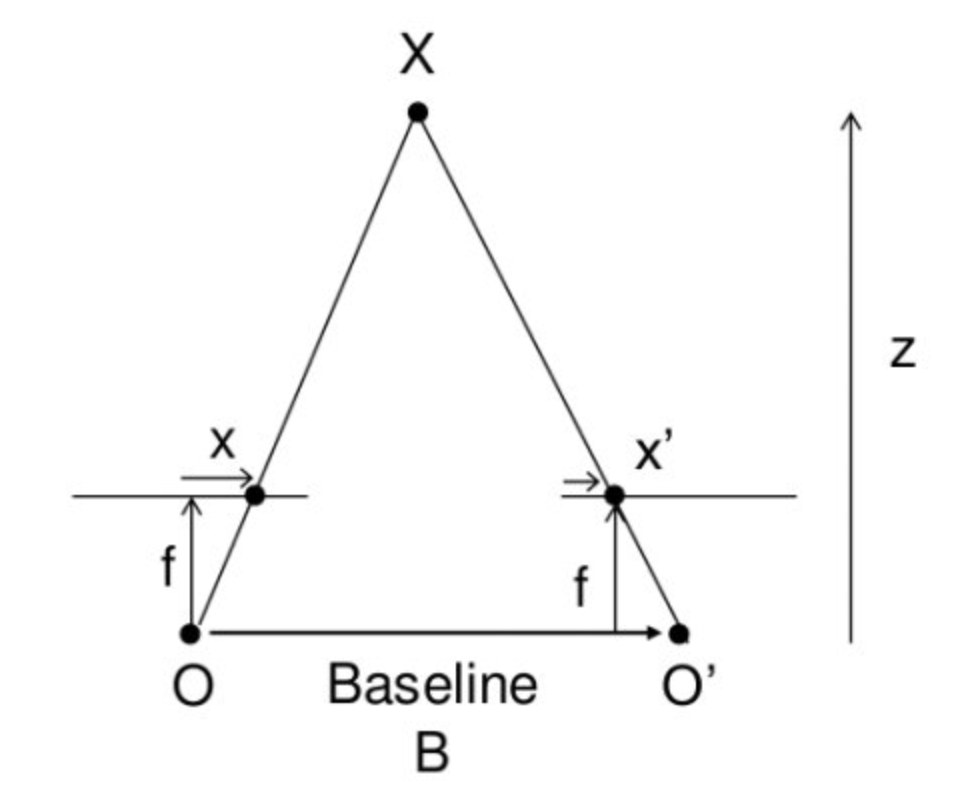
\includegraphics[width=0.5\textwidth]{disparity}
    \caption{Disparity and depth geometry}
    \label{fig:disp}
\end{figure}
This works by using "Sum of Absolute Difference" windows to find matching points between the left and right stereo-rectified images. 
This algorithm finds only strongly matching (high-texture) points between the two images. Thus, in a highly textured scene such as might occur outdoors in a forest, every pixel might have computed depth. 
In a very low-textured scene, such as an indoor hallway, very few points might register depth.\\
The algorithm operates in three stages:
\begin{enumerate}[label={\arabic*.}]
    \item Prefiltering to normalize image brightness and enhance texture.
    \item Correspondence search along horizontal scanlines (epipolar lines) using SAD window.
    \item Postfiltering to eliminate bad matches.
\end{enumerate}
The output of this operation will be a disparity image. 
This disparity map can in turn be used to estimate the relative depth of points and will be used to reproject them in 3D.
\subsection{3D Reprojection}
Reprojection of the entire disparity image to 3D is accomplished using the OpenCV function \texttt{cvreprojectImageTo3D} which operates on whole images.
This routine takes a disparity image and transforms each pixel's \((x, y)\) coordinates along with that pixel's disparity (i.e a vector \([x, y, d]^T\)) 
to the corresponding 3D point \((X/W, Y/W, Z/W)\) by using a reprojection matrix \(Q\) obtained from the \texttt{cvstereoRectify} function.
\begin{equation*}
    \begin{bmatrix} X \\ Y \\ Z \\ W \end{bmatrix} = Q \begin{bmatrix} x \\ y \\ \texttt{disparity} (x,y) \\ z \end{bmatrix}.
\end{equation*}
the matrix \(Q\) returned during rectification phase is the following \((4x4)\) matrix:
\begin{equation*}
    Q = \begin{bmatrix} 1 & 0 & 0 & -cx_1 \\ 0 & 1 & 0 & -cy \\ 0 & 0 & 0 & f \\ 0 & 0 & -\frac{1}{B} & \frac{cx_1 - cx_2}{B} \end{bmatrix}
\end{equation*}
where \(B\) is a horizontal shift between the cameras and $cx_1=cx_2$.
Furthermore \(-\frac{1}{B}\) is going to be \(-1\) because \(t\) obtained by SVD was a unit vector since no information on the distance between the cameras was provided.
\section*{Results}
Tests are conducted using a reflex camera (Canon EOS 600D) with a 50mm lens, 
the camera's intrinsic parameters are extracted during the calibration phase as explained in \ref{sec:calibration}, and stereo pairs are acquired
with the same camera. The stereo pairs portray different stationary objects, the position of the object in the scene must not change in time since the images
of the two views are not acquired simultaneously.
Here is shown an example of stereo pair (fig \ref{fig:stereo}), with relative computed disparity and 3D point cloud (fig \ref{fig:depth}).\\
\begin{figure}[h]
    \centering
    \begin{subfigure}{.5\textwidth}
      \centering
      \includegraphics[width=0.98\linewidth]{L10.JPG}
      \caption{Left view}
      \label{fig:10left}
    \end{subfigure}%
    \begin{subfigure}{.5\textwidth}
      \centering
      \includegraphics[width=0.98\linewidth]{R10.JPG}
      \caption{Right view}
      \label{fig:10right}
    \end{subfigure}
    \caption{Stereo pair}
    \label{fig:stereo}
\end{figure}
\begin{figure}[h]
    \centering
    \begin{subfigure}{.5\textwidth}
      \centering
      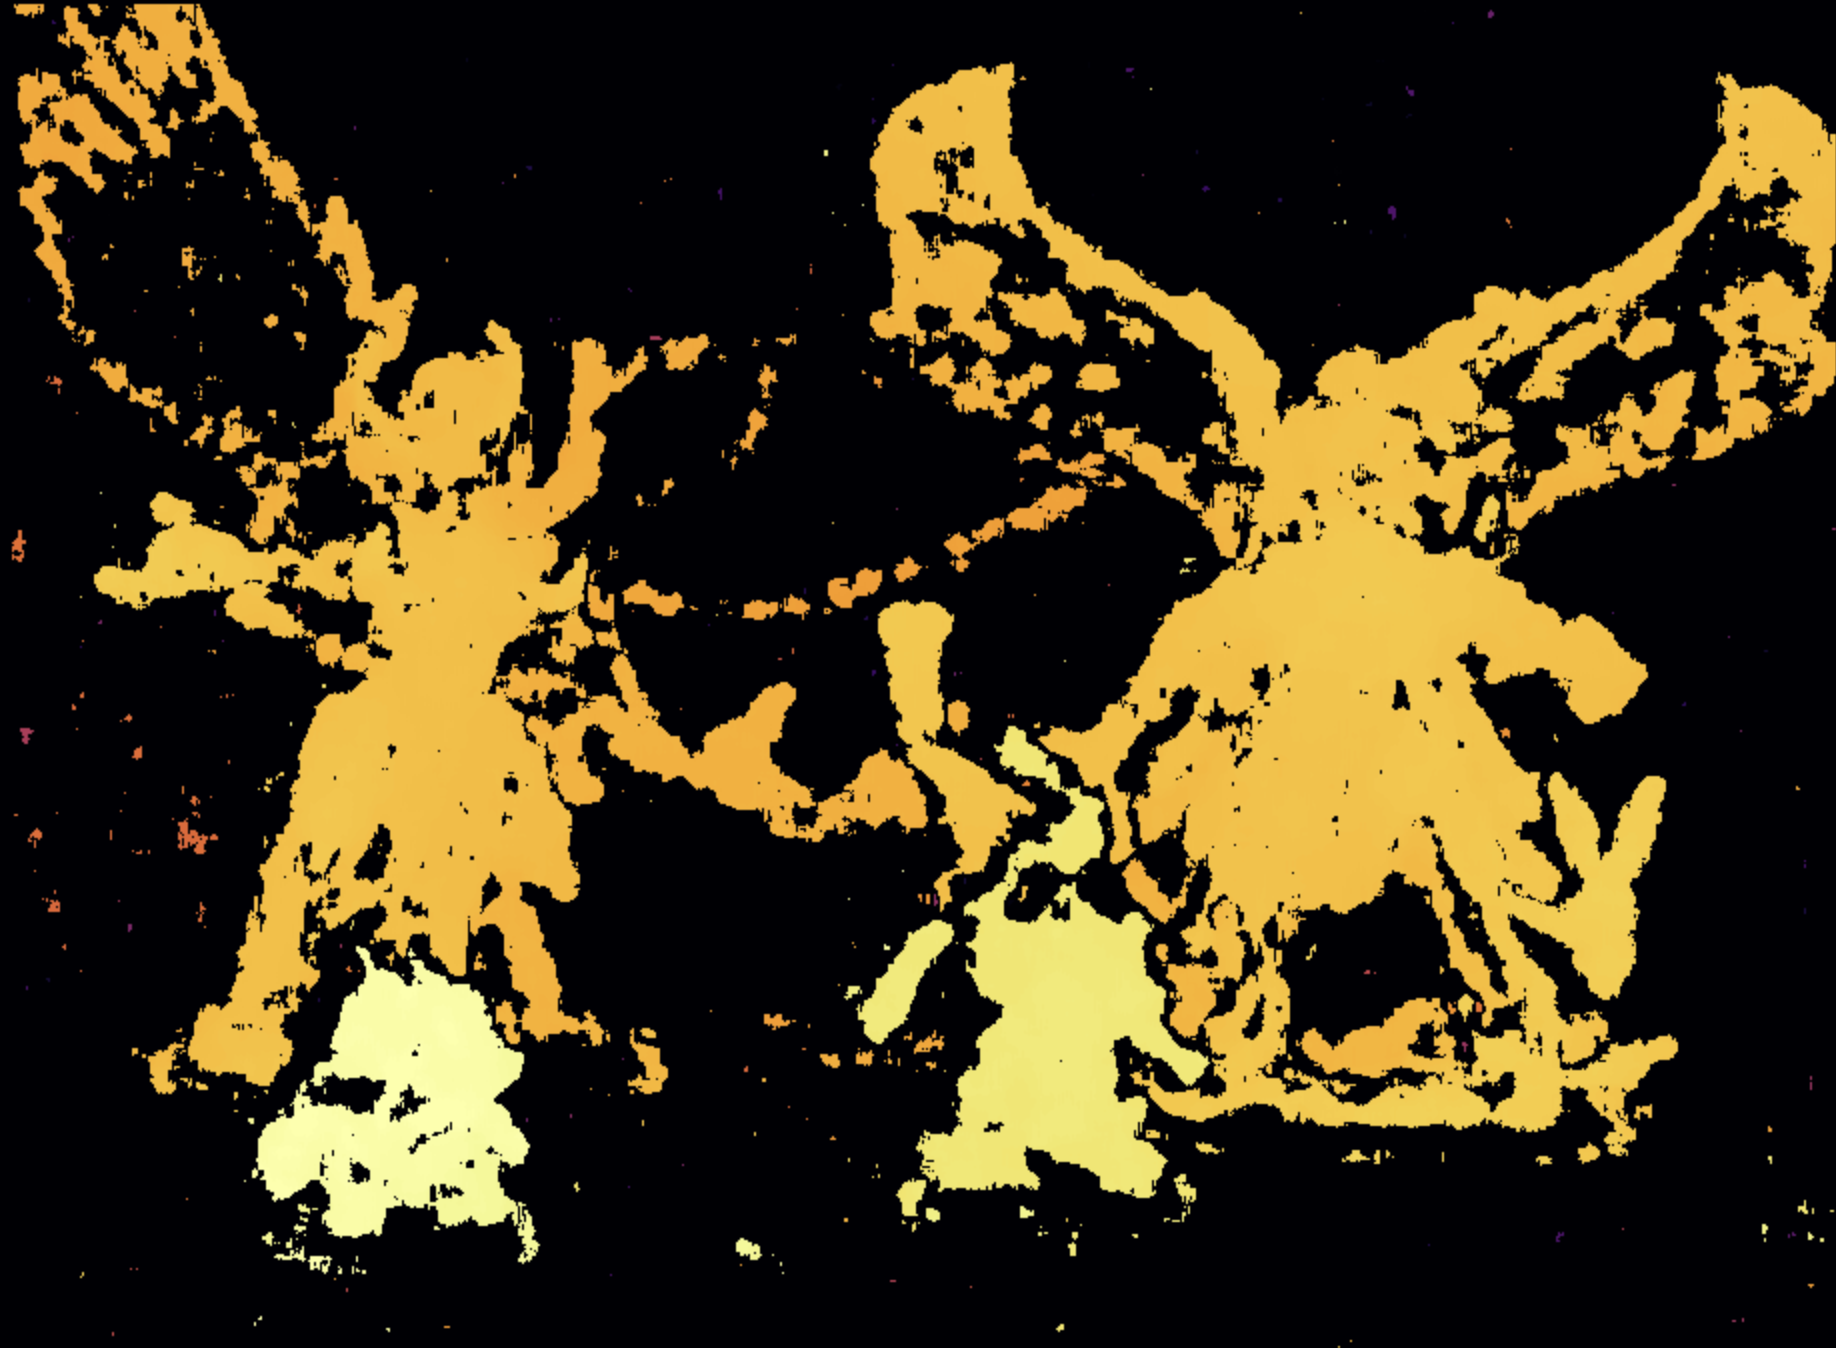
\includegraphics[width=0.98\linewidth]{disparitymap.png}
      \caption{Disparity image}
      \label{fig:disparityimg}
    \end{subfigure}%
    \begin{subfigure}{.5\textwidth}
      \centering
      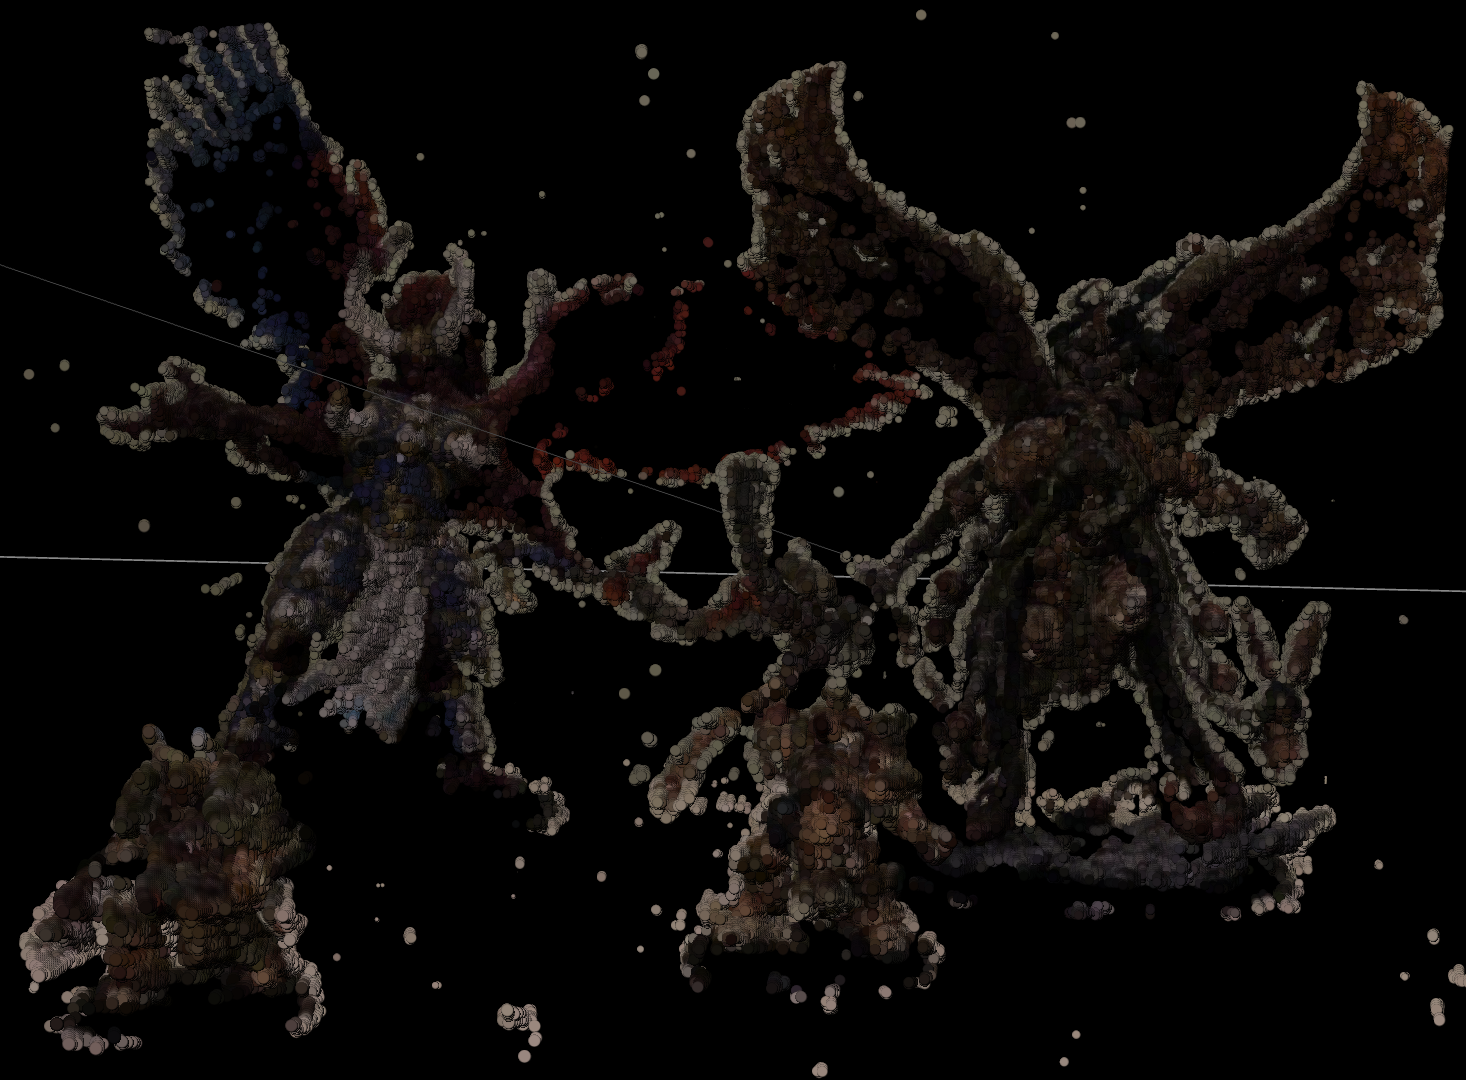
\includegraphics[width=0.98\linewidth]{pointcloud.png}
      \caption{Point Cloud}
      \label{fig:pointcloud}
    \end{subfigure}
    \caption{Disparity image and Point cloud}
    \label{fig:depth}
\end{figure}

The quality of the 3D reconstruction (up to scale) is strongly tied to the quality of estimation of the relative pose of the two cameras.
This fundamentally depends on how well the calibration process estimated the camera's intrinsic parameters and the number of good matches found by the matching algorithm
that will be used in the Fundamental matrix estimation procedure. The results are very sensitive to the quality and number of matches found.
More robust results can be obtained by acquiring the stereo images with two distinct calibrated cameras, in this case, the relative position of the two cameras is
computed during the calibration phase using a calibration pattern and can be more precise.
The considered approach can output correct 3D reconstructions of the scenes when the two image planes are close to parallel. 
When the angle or rotation of the second camera with respect to the first is not close to zero,
or the translation of one camera with respect to the first is not bound to the x-axis the rectification procedure fails to produce expected results
due to incorrect estimation of the relative pose. The next stereo block matching phase is unable to find correspondences if the two
images are not precisely rectified and as a result, the disparity cannot be computed.
As mentioned in the first section, being this a simple version of "Structure From Motion" limited to two views, a natural extension of this procedure is to consider
multiple views of the same stationary object. If the environment is relatively rich in recognizable features then 
it should be possible to compute correspondences between enough points — from frame to frame — to reconstruct not only the trajectory of the camera but also, indirectly, 
the overall three-dimensional structure of the scene and the locations of all the aforementioned features. 
Matching scene points from multiple views (not just two) could reconstruct a better 3D structure of the scene.
\section*{Deep Learning Approach}
For comparison purposes, a depth estimation method based on Deep Learning is explored in this section. The "ChiTransformer"\cite{chitransformer} method
approach fuses the two prevalent methodologies in deep learning based depth estimation, "Stereo Matching" and "Monocular Depth Estimation" (referred to as MDE). 
Stereo information can be injected into the MDE process to rectify and improve the estimation made from depth cues.
ChiTransformer adopts the recent Vision Transformer (ViT) as backbone and extends the encoder-only transformer to an encoder-decoder structure similar to
the ones for natural language processing.
The architecture is shown in figure (\ref{fig:chi}).
\begin{figure}[h]
    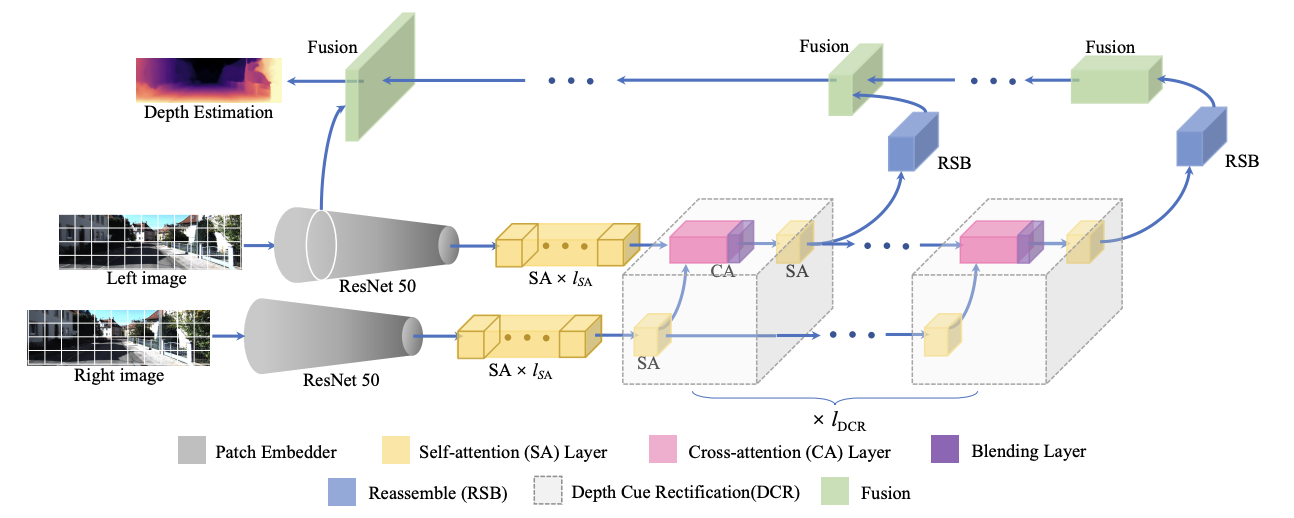
\includegraphics[width=0.9\textwidth]{Chi.png}
    \caption{ChiTransformer Architecture}
    \label{fig:chi}
\end{figure}
\printbibliography
\end{document} 